\documentclass{atistandalonetask}
\usepackage{atistandard}
\begin{document}
  \begin{atiTask}[
    title = Fluss durch einen Zylinder
  ]
  
 Gegeben sei ein Zylinder, dessen Grundkreis mit dem Radius $R$ in der $x$-$y$-Ebene und Mittelpunkt im Ursprung liegt. Seine Höhe betrage $H$. Weiterhin sei das Vektorfeld
 \begin{equation*}
 \vec{\phi}=\frac{1}{r}\vec{e}_r+\frac{1}{r}\vec{e}_\phi+\frac{1}{\sqrt{r^2+z^2}}\vec{e}_z
 \end{equation*}
 gegeben.
 \begin{atiSubtasks}
 \item Berechnen Sie den Fluss des Vektorfeldes durch die Oberfläche des Zylinders durch Ausführen eines Oberflächenintegrals.
 \item Berechnen Sie
 \[
 \iiint \divergence \vec{\phi}\;\D V,
 \]
 indem Sie über das Volumen des Zylinders integrieren.
 \item Begründen Sie, warum beide Ergebnisse nicht übereinstimmen.
 \end{atiSubtasks}

  \end{atiTask}
  \begin{atiSolution}
Loesung folgt
  %	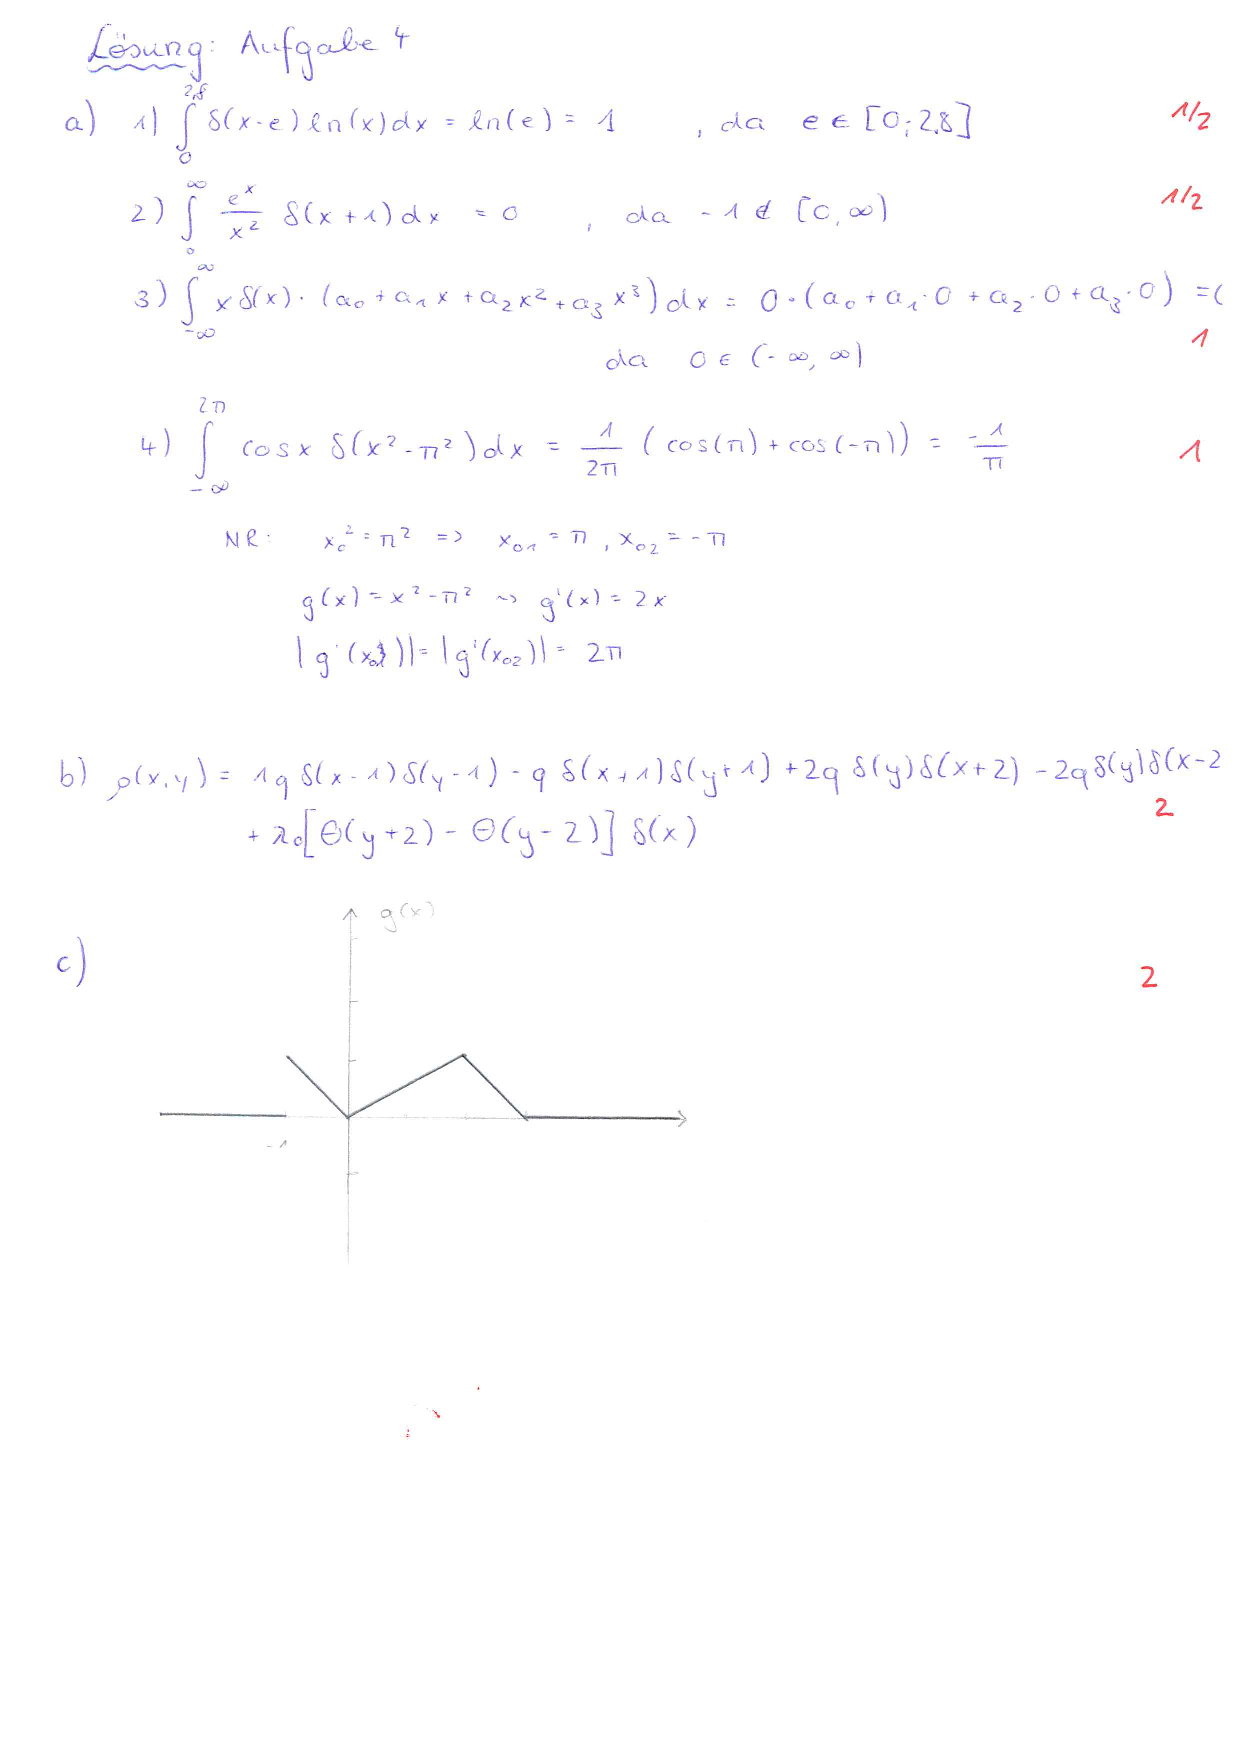
\includepdf[pages=-]{solution-delta_vii.pdf}
  \end{atiSolution}
\end{document}